\section{深度学习介绍}

\subsection{传统机器学习方法与局限性}

在之前的50年左右,传统的模式识别模型用手工定义的特征进行特征提取,通过对数据的分析选取可训分类器进行模型构建。 最近10年,借助现代计算机计算能力的提高和大数据量的爆发,神经网络方法得以重新广泛应用,在很多领域都达到非常好的效果, 我们称这种利用大规模网络进行模式识别方法为深度学习(Deep Learning), 也叫End-To-End Learning。不同于传统模型采用固定特征,或者固定kernel(核函数)进行样本度量; 深度学习采用可训特征(或可训的kernel), 然后将特征作为可训练的分类器输入, 进行训练, 如表\ref{Tab:dl_overview_compare}。

\begin{table}[ht]
\centering
  \begin{tabular}{|c||c|c|c|}
  \hline
   & 特征 & 分类器 & 特点\\
  \hline\hline
   传统方法 & 人工定义的特征 & 简单可训练分类器 & 特征设计费时,需强业务背景\\
  \hline
  深度学习 & 训练特征提取模型 & 复杂可训练分类器 & End-to-End learning,feature易操作\\
  \hline
  \end{tabular}
  \caption{深度学习与传统模式识别方法}
  \centering \label{Tab:dl_overview_compare}
\end{table}

历史上,第一个有学习功能的机器为1960年提出的Perceptron\cite{rosenblatt1960perceptron},也是神经网络的一个基本单元。 Perceptron是一个简单特征提取器上加载的一个线性分类器: 


\begin{equation}
\label{Eq:Perceptron}
y=sign(\sum_{i=1}^N{w_iF_i(x)}+b)
\end{equation}


其中$x$为数据,$F_i(x)$为x的第i个特征,$w_i$为相应的特征权重参数, b为常参数, $sign$为分类器的非线性函数,对于二类分类,$sign$函数将结果映射到(0,1)。

\begin{figure*}[htb]
  \centering
  % Requires \usepackage{graphicx}
  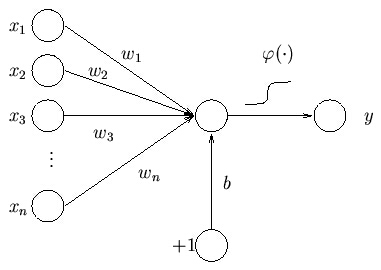
\includegraphics[scale=0.9]{Pictures/CNN/perceptron.jpg}\\
  \caption{Perceptront图例}\label{fig:perceptron}
\end{figure*}

目前最普及的实际应用也用到了线性分类器的一些变种,或者叫模板匹配(template matching)。 但是由于其底层的特征提取器需要反映特定信号的特点, 所以需要由特定领域专家来设置。 比如图像处理领域, 对于不同任务( 图像分类, 图像分割, 图像跟踪等), 所要求的特征就各不相同, 需要针对特定任务定义图像特征。 此外,传统方法也很难设计kernel, 从而不容易表达对距离的度量,仍然以图像来说,最简单的距离度量思路是对应像素相减,但是这显然不能表达图像语义层的相似信息。

为了能使特征更加灵活而且不过多依赖于专家指定的特征, 很多方法提出, 可以先人为定义简单特征, 然后通过无监督学习方法进一步得到中间层特征, 将其输入分类器进行最后分类。
典型的无监督特征学习方法如混合高斯模型\cite{jeong2004image,gray2001gauss,gauvain1992bayesian,reynolds2000speaker,reynolds1995robust, zivkovic2004improved,lee2005effective,yang1999gaussian}, K-Means\cite{liu2007computational,netzer2011reading,coates2011text,dy2004feature,coates2012learning}, 和Sparse Coding\cite{yang2009linear,boureau2008sparse,coates2011importance,coates2011analysis,gao2010local,mairal2010online}。 但这仍然不能解决以下几个问题:

\begin{enumerate}
	\item 建立传统模型代价大\\
	对每个领域,每个任务都需要设计特征。即便有了中间特征层进行无监督的特征选择, 庞大冗余的基础特征的设计也是耗时费力的。 随着工业界对不同任务的需求, 需要建立很多基础特征、 模型, 代价也很大。
	\item 无法很好地利用计算性能\\
	计算机性能的大幅提升本可以用来帮助加速机器学习, 但传统机器学习需要人工定义模型, 从而使模型规模受限,不能很好地利用计算性能和大量数据。 
	
	\item 人工定义特征效果欠佳\\
	目前, 自动学习的特征已经在图像、语音等很多领域强于人工定义的特征。 而且如果需要增加特征维度进行大规模学习就需要再手工定义更多特征, 而不能简单地够自动按比例扩大。
	
\end{enumerate}


\subsection{深度学习方法介绍}

深度学习是近几年来很热的机器学习算法, 在语音识别,计算机视觉,自然语言处理等领域打破了维持了多年的竞赛记录。以最典型的时序模型——语音识别的发展为例, 在1980年代早期, 主要应用Dynamic time Warping (DTW)\cite{juang1984hidden,myers1981comparative,rabiner1978considerations,berndt1994using}, 输入底层特征,通过无监督学习所得中间层特征输入分类器进行分类。 1985年后, \cite{huang1990hidden,rabiner1989tutorial,rabiner1986introduction}提出在中间层用隐马尔科夫模型描述一个序列出现的概率,得到进一步改进。 2010年左右, 使用深度神经网络进行逐层有监督学习达到最佳效果\cite{waibel1989modular,nakamura1989speaker}。


同传统方法的基本方法类似, 深度学习也是从数据分别生成底层特征, 中间层特征, 最后加入高层特征, 输入分类器进行分类, 即学习数据的结构化表示。 其形式化表示为:
\begin{equation}
y=f(W^kf(W^{k-1}f(...f(W^0X)...)))
\label{Eq:dl_formulation}
\end{equation}
其中, W为权重参数,k为层数,$W^iX$为输入X的线性表示, $f$为非线性函数, 如$tanh$ 函数。 深度学习就是优化$y$与groundtruth之间的距离,使之最小化。 从图像角度, 如图\ref{fig:feature_level}所示\cite{zeiler2014visualizing,zeiler2013stochastic},图中(a),(b),(c)分别为自动学得的底层特征,中层特征和高层特征, 其中底层特征学习图像的浅层特征,在所有类别中共享, 如(a)中,学到的特征类似Gabor滤波器所提取的边缘特征\cite{ngiam2010tiled,shi1998gabor}, 从中间层到高层依次学习图像更深层的语义特征, 如有语义的显著图像区域, 高层特征更为稳定,也具有类属性。  从自然语言处理的角度, 初始输入为字符, 从底层向上依次学习单词, 短语, 长句, 文章。

\begin{figure*}[htb]
  \centering
  % Requires \usepackage{graphicx}
  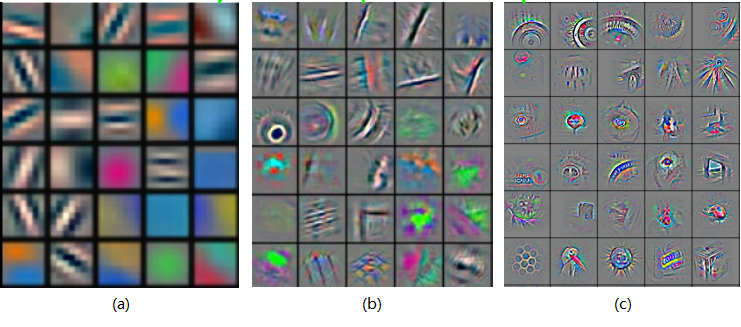
\includegraphics[scale=0.9]{Pictures/CNN/low_mid_high_feature.png}\\
  \caption{各层次feature}\label{fig:feature_level}
\end{figure*}


除了自动学习特征外, 深度学习和传统模型还有一个重要区别就是“深”。 一般来说, 深度结构由多层含参的非线性模型组成, 以形成特征的层次结构。
在\cite{bengio2007scaling,bengio2009learning}中讨论了深度模型的必要性。 浅层结构以现在的kernel machine\cite{scholkopf1999advances}为例, 如Support Vector Machine(SVMs)\cite{boser1992training,cortes1995support}。 这些方法定义特征
为一系列kernel函数连接而成的向量, 在训练数据中进行模板匹配, 如式\ref{Eq:kernel_fea_vec}所示。

\begin{equation}
	\label{Eq:kernel_fea_vec}
	\varphi(x) = [k(x,\mu_1),k(x,\mu_2),...,k(x,\mu_n)]
\end{equation}

式中, $\mu_i$为数据样本的一部分, 即模板样本; $\varphi(x)$为样本$x$的特征。 而后$\varphi(x)$通过线性组合进行分类:


\begin{equation}
	\label{Eq:kernel_predict}
	F(x) = W^T\varphi(x)
\end{equation}

可见, kernel方法就是一个简单的模板匹配层连接一个线性函数层, 由于方法中模板都是从原始训练数据中提取而得, 所以kernel machine的第一层
可视作一种简单的无监督方法, 只有式\ref{Eq:kernel_predict}中参数$W$的学习为有监督部分,没有涉及特征的层次结构, 因此不是深度模型。 同样,只有一个隐层的模型(如multilayer perceptron)也不算深度模型。 又如分类回归树(Classification and Regression Tree, CART), 其中所有决策都是在输入空间定义的, 同样没有根据特征的层次结构进行学习, 因此也不属于深度模型。 虽然有一些理论保证浅层结构可以以任意精度拟合任何复杂函数\cite{hornik1989multilayer,hecht1989theory,komolgorov1956representation}, 它们却无法保证特征的高效表征。 而深度模型可以从根本上通过简单设置网络结构更有效地表示特定函数。 最典型的深度结构就是有多个隐层的神经网络, 其中每个隐层节点之间的连接权重(如图\ref{fig:perceptron}中的$w_i$)都是通过有监督学习而来的, 因此可以很好地表征数据属性。



\begin{figure*}[htb]
  \centering
  % Requires \usepackage{graphicx}
  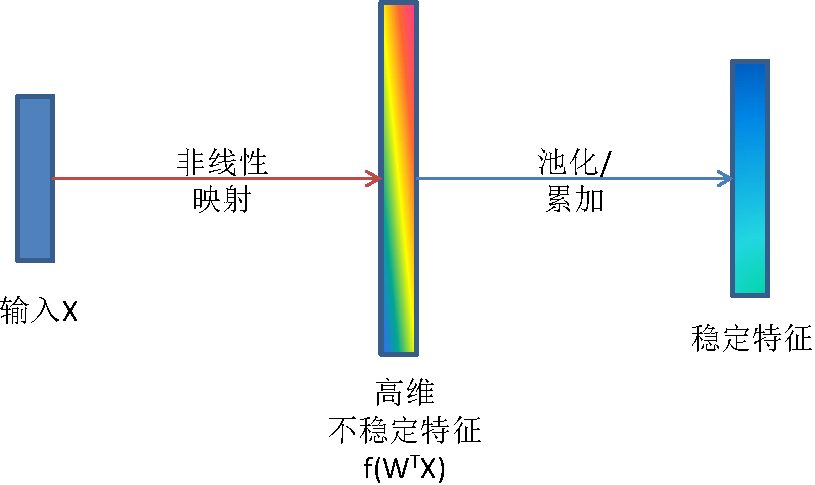
\includegraphics[scale=0.8]{Pictures/CNN/invariant-feature-crop.pdf}\\
  \caption{稳定特征生成方法}\label{fig:invariant_feature_learning}
\end{figure*}


神经网络在1940年代就开始了相关研究\citep{mcculloch1943logical,hebb1949organization}
, 但早期提出的神经网络多为线性回归的变种, 没有很大突破。 1965年, \cite{ivakhneko1995review}提出了第一个深度学习模型——Group Method of Data Handling (GMDH), 它通过回归方法进行网络训练, 再通过决策正则化去掉多余节点。 直到现在仍有很多应用以GMDH为基本框架, 如\cite{ikeda1976sequential,farlow1984self,madala1994inductive,kordik2003modified,witczak2006gmdh,
kondo2008multi}。 1960年代,受神经科学的启发, 神经网络也随之发展。 当时神经科学在猫的视觉皮层发现了简单细胞和复杂细胞, 简单细胞对局部视觉特征(如边缘的方向)敏感, 会做出一定响应; 而复杂细胞相对简单细胞表现出更为鲁棒的响应, 即不受空间变化的影响, 可以在视网膜一块邻域区域中选出简单细胞的一个输入作为输出。 受此启发, 1979年 \cite{fukushima1979neural} 第一次在Neocognitron中引入了类似卷积神经网络的概念。 Neocognitron是为手写体识别提出的一个有层级结构的多层神经网络, 它不仅可以识别训练样本中的模式, 还可以识别训练样本经过平移, 旋转或其他变换后的模式。 其结构和现在我们用到的前向卷积神经网络比较相似, 层间连接也应用了现在我们常用卷积神经网络类似的部分权值共享(详见第\ref{sec:CNN}节)。 只是, Neocognitron通过无监督学习, 根据样本获得不同的pattern, 而不同于现在的有监督误差反传方法。 此外还有一些小差别,比如在pooling策略上, Neocognitron采用空间域平均, 而且虽然Neocognitron的层级较深, 但是它并没有在效果中考虑到深层带来的效果。 



由于90年代计算资源和数据量受限, 当隐层层数大于2的时候深度网络训练困难\cite{tesauro1992practical}, 所以之前神经网络的研究工作主要集中于浅层结构。 随着现在数据量的爆发, 神经网络的研究变得重新热门起来。 其基本思想是学习具有不变性的特征, 即,将输入数据映射到一个非线性的高维空间,使数据变得可分。 如\ref{fig:invariant_feature_learning}所示,输入经过非线性函数的映射到高维特征, 使数据变得可分, 但是这样的高维特征可能由于训练数据间差异导致不稳定,所以将高维数据中相似语义信息的成分通过池化(pooling)或累加等方法整合到一起, 形成稳定特征。





\subsection{深度神经网络结构与训练}

\subsubsection{网络结构}\label{sec:network_architecture}

从网络结构来分, 神经网络有前向网络(包括multilayer neural nets\cite{kuurkova1992kolmogorov,
hornik1989multilayer,hornik1991approximation}和 convolutional nets \cite{lecun1995convolutional,krizhevsky2012imagenet},), 回馈网络(包括 stacked sparse coding\cite{yu2011learning}, deconvolutional nets\cite{zeiler2010deconvolutional})和双向网络(包括 deep boltzmann machines\cite{salakhutdinov2009deep,
srivastava2012multimodal,goodfellow2013multi}, stacked auto-encoder\cite{gehring2013extracting,vincent2010stacked,vincent2008extracting})三类\cite{lecun2013deep}。 目前, 前向网络使用最广, 如图\ref{fig:feed_forward}所示为一个前向网络的示意图。 

\begin{figure*}[htb]
  \centering
  % Requires \usepackage{graphicx}
  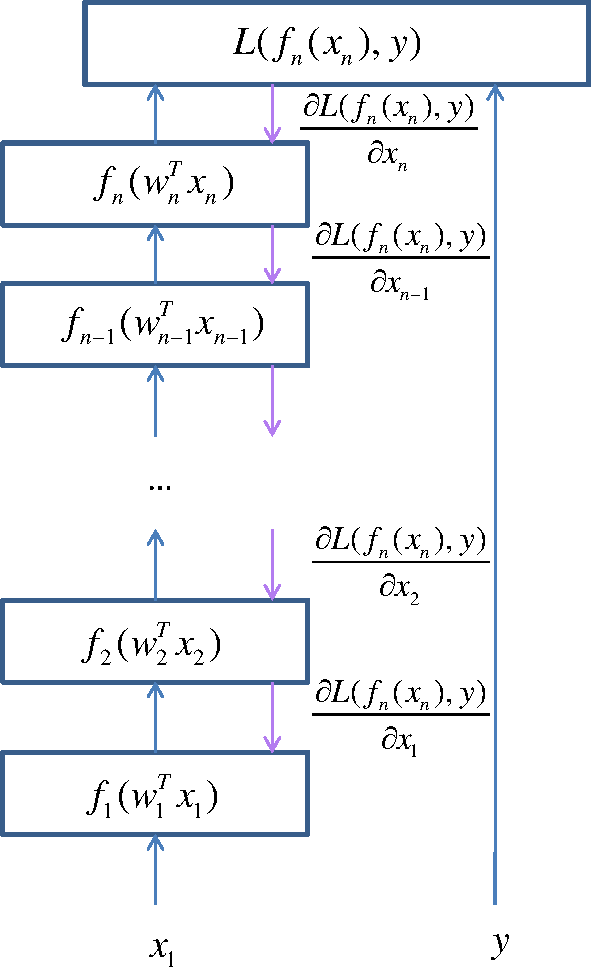
\includegraphics[scale=0.9]{Pictures/CNN/feed-forward-crop.pdf}\\
  \caption{前向网络的网络结构}\label{fig:feed_forward}
\end{figure*}

其中, $x_i$表示第i层的输入, 整个网络的输入为$x_1$; $w_i$表示第i层的参数, $w_i^Tx_i$得到$x_i$的线性组合; $f$为非线性函数, 每一层通过非线性函数将输入数据映射到下一层, 如图中蓝色箭头所示。 经过每一层非线性映射$f_i$的刀下一层输入,即
\begin{equation}
 x_i = f_{i-1}(w_{i-1}^Tx_{i-1})
\end{equation}

给定$x_1$对应的样本label $y$,我们的目标函数为$L(f_n(x_n),y)$, 其中$L$为损失函数。 常见的损失函数有平方损失, 指数损失, 对数损失等。 



\subsubsection{网络训练与误差反传}

自从1960年以来,不断有文章\cite{griewank2012documenta,director1969generalized,gray1965effect,bellman1962applied,
kelley1960cutting,bryson1961diffraction,}从变分法中的欧拉-拉格朗日方程出发讨论如何利用梯度下降(gradient descent, 也叫steepest descent)的方法\cite{hadamard1908memoire} 来进行神经网络中多层非线性可导函数的优化。
在这样的神经网络中, 可以通过链式法迭代地则对每个神经元求导\cite{bellman1962applied}。 之后,1970年, 误差反传算法(back-propagation algorithm, BP)\cite{hecht1989theory,goh1995back} 首次在Linnainmaa的硕士毕业论文\cite{linnainmaa1970representation}中提出, 其中描述, 误差反传算发可以高效应用于任意神经网络结构。 此后BP迅速应用到神经网络的训练中, 并实现了给定可导函数自动求解导数和BP\cite{speelpenning1980compiling}。 其基本思想如下: 由图\ref{fig:feed_forward}和式\ref{Eq:dl_formulation}, 在前向算法中从输入到输出经过了一系列非线性可导函数$f$的映射。  每次针对一个样本, 计算出其输出和样本真实label之间的loss$L$, 然后自上而下逐层更新权重参数$w$(如图中向下的紫色箭头所示), 使得当前误差可以减小。 用所有样本依次对权重做完更新后叫做一轮迭代。 不断做n轮迭代, 直到全局loss降到某个预设阈值, 这时网络就已经学好了。 其中, 对 $w_i$ 更新权重时采用梯度下降的方法:

\begin{equation}
\label{Eq:gradient}
	\Delta w_i = -\gamma \frac{\partial L}{\partial w_i}
\end{equation}

\begin{equation}
\label{Eq:gradient_descent}
	w_i = w_i + \Delta w_i
\end{equation}

式\ref{Eq:gradient}中, $\gamma$表示学习率, 就是每一步朝梯度下降方向走的步长, 是一个正的常数。 注意这里的负号表示loss是朝梯度下降的方向走。 式\ref{Eq:gradient_descent} 表示$w_i$ 每一步的更新。 但是$L$的表达式中难求对每个$w_i$的导数, 这里我们用$net_{j}$表示第j个隐层节点, 有

\begin{equation}
	net_j = \sum_i{w_{ij}o_i}
\end{equation}

即上一层输出到该节点的线性组合,其中$o_i$表示节点i的输出, $w_{ij}$表示节点i到j之间的连接, 有$o_{j} = f(net_j)$, 则$L$对$w_{ij}$的导数如式\ref{Eq:bq_basic}。


\begin{equation}\label{Eq:bq_basic}
\begin{split}
\frac{\partial L}{\partial w_{ij}} 
&= \frac{\partial L}{\partial net_j}\cdot \frac{\partial net_j}{\partial w_ij}\\
&= \frac{\partial L}{\partial net_j}\cdot \frac{\partial \sum_k{w_{kj}o_k}}{\partial w_ij}\\
&= \delta_{j}\cdot o_i
\end{split}
\end{equation}

其中$o_i$为前向过程中第i层的输出, $\delta_j = \frac{\partial L}{\partial net_j}$i为第i层中从后向前传递的错误, 我们称之为反向传播误差(backpropagated error)。 由公式\ref{Eq:gradient},\ref{Eq:gradient_descent}和\ref{Eq:bq_basic}可知, i,j节点之间的权重的参数$w_{ij}$更新由节点j在输出端的反向传播误差乘以节点i的输出$o_i$(也就是节点j的输入端)而得, 如图\ref{fig:update_weight} 所示, 黑色线条表示前向通路, 红色线条表示反向传回的误差$\Delta w_{ij}$。

\begin{figure*}[htb]
  \centering
  % Requires \usepackage{graphicx}
  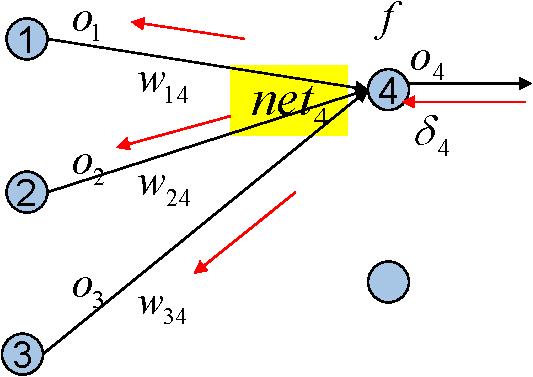
\includegraphics[scale=0.8]{Pictures/CNN/weight_update-crop.pdf}\\
  \caption{误差反向传播示意图}\label{fig:update_weight}
\end{figure*}


对于多层网络, 考虑如何计算反向传播误差$delta_{i}$。 对于整个网络的输出单元$net_n$, 可以直接算得$\delta_n = \frac{\partial L}{\partial net_n}$, 例如对于$L$取square loss的情况, 有


\begin{equation}
\begin{split}
&	L(y,net_n)=\frac{1}{2}(net_n-y)^2 \\
&	\delta_n = \frac{\partial L}{\partial net_n} = net_n - y
\end{split}
\end{equation}


对于隐层节点$net_j$, 通过链式法则求导可得, 如图\ref{fig:update_weight_2}和公式\ref{Eq:hidden_update}所示。 
\begin{equation}\label{Eq:hidden_update}
\begin{split}
\delta_j
	&=\frac{\partial L}{\partial net_j}\\
	&=\sum_{k}\frac{\partial L}{\partial net_k}\cdot \frac{\partial net_k}{\partial net_j}\\
	&=\sum_k \delta_{k} \cdot \frac{\partial \sum_i{w_{ik}o_i}}{\partial net_j}\\
	&=\sum_k \delta_{k} \cdot \frac{\partial \sum_i{w_{ik}f(net_i)}}{\partial net_j}\\
	&=\sum_k \delta_{k} \cdot w_{jk} f'(net_j)
\end{split}
\end{equation}

\begin{figure*}[htb]
  \centering
  % Requires \usepackage{graphicx}
  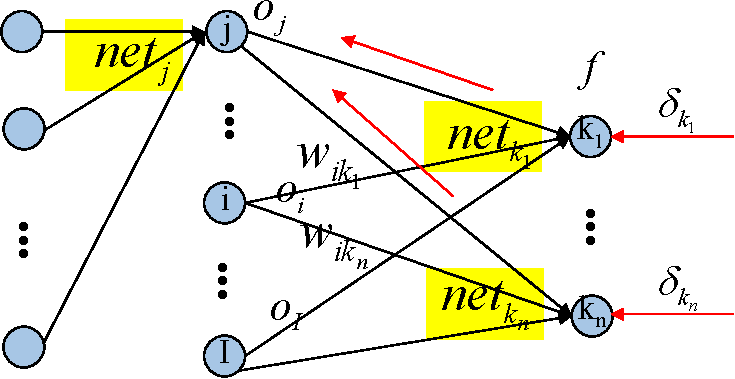
\includegraphics[scale=0.8]{Pictures/CNN/weight_update_2-crop.pdf}\\
  \caption{$\frac{\partial L}{\partial net_j}$链式法则示意图}\label{fig:update_weight_2}
\end{figure*}

这样就可通过将误差逐层传递训练网络了。 整个算法流程如算法\ref{algo:BP_basic}所示。 在每一次迭代中, 首先前向计算出每个节点的输入$net_j$ 和输出$o_j$(见3~6行。 然后用误差反传算法, 在输出层直接用损失函数对节点求导计算反传误差(9-11行), 其他隐层节点用公式\ref{Eq:hidden_update}计算反传误差(12-14行),最后更新权重参数(15-18行)。


\renewcommand{\algorithmicrequire}{ \textbf{Input:}}      %Use Input in the format of Algorithm
\renewcommand{\algorithmicensure}{ \textbf{Output:}}     %UseOutput in the format of Algorithm
\begin{algorithm}
\caption{前向网络的误差反传算法}
\label{algo:BP_basic}
\begin{algorithmic}[1]  
\Require Data $x$, Label $y$
\Ensure  updated weight $w$
\For{t=1...T} \% 迭代次数
	\State \textbf{\textit{\% forward propagate}}
	\ForAll{unit $j$ not $\in$ input layer}
	\State $net_j \leftarrow \sum_i w_{ij}o_i$
	\State $o_j \leftarrow f(net_j)$
	\EndFor
	\State 
	\State \textbf{\textit{\% back propagate error}}
	\ForAll{ unit $k \in $ output layer }
		\State $\delta_k \leftarrow \frac{\partial L}{\partial net_k}$	\%直接求导计算	
	\EndFor	
	\ForAll{ unit $j \in $ hidden units }
		\State $\delta_j \leftarrow f'(net_j)\sum_k{w_{kj}\delta_k}$ \%根据公式\ref{Eq:hidden_update}
	\EndFor	
	\ForAll{ weight $w_{ij}$ } \%根据公式\ref{Eq:gradient_descent}和\ref{Eq:bq_basic}更新权重参数
		\State $\Delta w_{ij} \leftarrow \frac{\partial L}{\partial w_{ij}} = \delta_{j}\cdot o_i$
		\State $w_{ij} \leftarrow w_ij + \Delta w_{ij}$
	\EndFor
\EndFor
\end{algorithmic} 
\end{algorithm}


BP尽管在理论上支持深度网络的训练, 但是实际应用中BP一般只对较浅的模型有效\cite{schmidhuber2015deep}, 因此提出了很多BP的改进算法,如:

\begin{enumerate}
\item 关于BP加速\\
为了加速BP, Rumelhart等人在1986年引入动量(momentum)\cite{rumelhart1985learning}; Fahlman向线性化的激活函数$f$的斜率加入ad-hoc常数\cite{fahlman1988empirical}; Sperduti 
不但对x进行梯度下降,同时对梯度参数也进行梯度下降; \cite{sarkar1995methods} 将不同的bp加速策略做了比较。
\item 关于BP学习率\\
一般地, BP有两种学习率设定方法: 全局学习率 \cite{lapedes1988neural,vogl1988accelerating,lecun1993automatic} 和对每个权重都设一个自己的学习率\cite{jacobs1988increased,almeida1990speeding}。 在线学习中,$vario-\eta$\cite{neuneier1998train} 算法设置学习率与当前节点梯度的标准差成反比, 从而可以不受随机权重初始化的影响。

\item 如何增强模型普适能力(generalization)\\
为了提高模型的generalization,一些方法采用weight decay \cite{hanson1989comparing,weigend1991generalization}, 它本质上是一种正则化方法, 通过在loss function中加入权重参数的平方项来鼓励更小的权重, 惩罚大权重。 在线性模型中, 这种方法就是ridge regression。 加入weight decay一来可以限制模型的复杂度, 防止模型过拟合, 二来如果激活函数不能将输出规范化到输出应在的范围内, 大权重很可能让输出远远大于数据范围。 此外,大权重还会陷入Bias/Variance Dilemma\cite{geman1992neural}, 导致输出数据波动很大。 Hinton等人\cite{hinton1993keeping}从贝叶斯角度解释了weight decay可以从weight的高斯先验假设中得来, 证明了这不是一个简单的猜想。 另一些方法通过在weight中加其他先验实现同样的功能\cite{hastie1990generalized,hastie2009elements,mosteller1968data,mackay1992evidence}。

\end{enumerate}

	
总结一下, 误差反传算法通过求损失函数对每个权重参数的导数对它们进行更新, 更新过程从输出端到输入端依次向下传递误差。 与数值差分相比, 误差反传方法更适应计算机运算, 而且计算更为高效。 在实际应用中, BP也有一些条件, 当问题定义的复杂度很高, 不能写出解析解, 但是确定有解的时候我们采用BP进行网络优化。 否则可能用传统方法或者查找表方法会更为简单精确, 具体问题具体分析。 


在第\ref{sec:network_architecture}节中这三种为网络结构中, 卷积神经网络属于广泛应用的前向神经网络。 我们将在第\ref{sec:CNN}节中介绍卷积神经网络的结构与训练过程, 在第\ref{sec:cnn_configure}节中介绍我们的数据与网络配置, 最后在第\ref{sec:cnn_experiment}中给出实验结果。


\section{卷积神经网络}\label{sec:CNN}
在上一节中我们已经提到, 卷积神经网络(Convolutional Neural Networks, CNN)是前向网络的一种, 其原型始于1979年Fukushima提出的Neurocognitron\cite{fukushima1979neural}, 但在后期经过了很多改进。 1989年, Lecun将误差反传算法应用于带有共享权值(详见第\ref{sec:cnn_arch}节)的卷积神经网络进行训练\cite{lecun1989backpropagation}, 这一工作的内容是现在我们前向神经网络的重要部分。 在20世纪90年代, CNN在指纹识别\cite{baldi1993neural}、 人脸识别\cite{lawrence1997face}、 语音识别\cite{abdel2012applying}、 物体识别\cite{nebauer1998evaluation}、 文档识别\cite{lecun1998gradient} 上的应用相继出现出现并予以商用。  

近几年来, 随着计算机计算能力的增强和数据量的激增, 卷积神经网络在各个领域的应用更为广泛, 也得到了更好的效果。 以机器视觉领域为例, 09年, Turaga(MIT)等人用学习的方法, 以卷积神经网络为模型训练生成相似图\cite{turaga2010convolutional}, 使得和传统人工定义分割函数的方法相比,分割精度有了很大提升。 2011年, Sermanet(NYU)和Lecun将CNN应用于交通标志分类\cite{sermanet2011traffic}, 在GTSRB竞赛数据集\cite{stallkamp2011german}上达到99.17\%的最高准确率, 超过人的识别能力。 对于图像分割任务, 很多算法需要首先生成一张相似图(affinity graph)然后在其上做分割。 2012年, Alex Krizhevsky(Google)在ImageNet\cite{deng2009imagenet}上应用深度卷积神经网络进行图像分类\cite{krizhevsky2012imagenet}。 该任务要将130万高清图像分成1000类, Krizhevsky采用5层卷积层, 共50万个神经元节点,6000万个参数进行训练,达到了当时图像分类的最佳效果。 2014年, Taigman(Facebook)等人应用卷积神经网络建立了DeepFace\cite{taigman2014deepface}, 在包含4000多人的4百万人脸图像数据集上进行训练, 在LFW数据集\cite{huang2007labeled}上进行人脸识别, 结果达到97.35\%的识别率, 近乎和人的识别水平相当。 整个过程为检测人脸->对齐->3d人脸表征->分类, 其中分类用的是多达1.2亿个参数的9层非标准卷积神经网络。 同年, Simonyan(Oxford)等人将深度卷积神经网络应用到视频进行行为识别\cite{simonyan2014two}。 他们提出了一个双CNN框架, 分别在时间和空间方面各应用一个CNN, 并证明再多帧的深度光流上应用ConvNet可以在有限数据集上达到很好的效果。 Toshev和Szegedy(Google)用深度神经网络进行人体姿态估计\cite{toshev2014deeppose}。 该方法在CNN上实现一个回归问题, 回归目标为人体节点(如关节处), 然后将多个这样的深度神经网络级联, 在姿态估计方面达到了目前最佳的准确率。 


此外, DeepMind团队(Google)\cite{mnih2013playing}在卷积神经网络上进行增强学习,实现了机器自动打游戏。 Ciresan\cite{ciresan2013mitosis}将深度神经网络应用于医学图像, 进行癌细胞检测。  自然语言处理方面, Denil(Oxford)等人通过将文档嵌入一个低维向量空间来提取文档语义信息并做归类,  该模型基于卷积神经网络, 在语义级别和文档级别同时学习卷积核。在框架方面, 2014年, Goodfellow在神经网络中提出了一个估计生成模型的框架\cite{goodfellow2014generative}, 通过同时学习两个相互对立的模型, 一个生成模型G拟合数据分布,一个判别模型D估计样本从训练数据得到(而不是从G得到)的概率。最终目标最大化D犯错误的概率(即让G尽可能地模拟原始数据分布), 其中G和D都是多层perceptron。 神经科学方面, Cadieu(MIT)将卷积神经网络应用下颞叶皮层信号的建模\cite{cadieu2014deep}, 揭示了下颞叶皮层在基于视觉的物体识别任务上对信息的表征能力。 也有工作将卷积神经网络应用于功能性磁共振成像(fMRI)数据大脑神经信号解码\cite{firat2014learning}, 结果和其他模式分析技术相比有所提高。 Barnickel等人基于卷积神经网络提出了SENNA, 一个快速精确地从生物类文献中提取分析予以相关性的神经网络\cite{barnickel2009large}。 

在第\ref{sec:introduction_p300}节中我们已经介绍过P300神经信号的产生及其对应的P300检测任务。 受以上文章启发, 本文中采用卷积神经网络为P300信号建模, 并应用于P300信号检测。 下面, 我们先来看一下卷积神经网络是如何工作的。


\subsection{CNN网络结构}\label{sec:cnn_arch}

\paragraph{卷积层}

如图\ref{fig:feed_forward}所示, 卷积神经网络也是一个层级结构的前向神经网络。 除了输入层和输出层, 中间的隐层的目标是从原始数据学得一系列非线性组合, 使得可以很好地结合当前任务表征信号。 以图像为例, 输入为像素级数据, 每个像素本身不含有太多信息, 但是组合起来所得到的更高级别的特征可以表示物体类别等信息。 尽管我们的神经信号不同与图像信号, 但是文本分析\cite{collobert2008unified}, 语音识别等其他任务都受了图像的启发, 因其方便可视化, 所以我们采用图像进行解释。


\begin{figure*}[htb]
  \centering
  % Requires \usepackage{graphicx}
  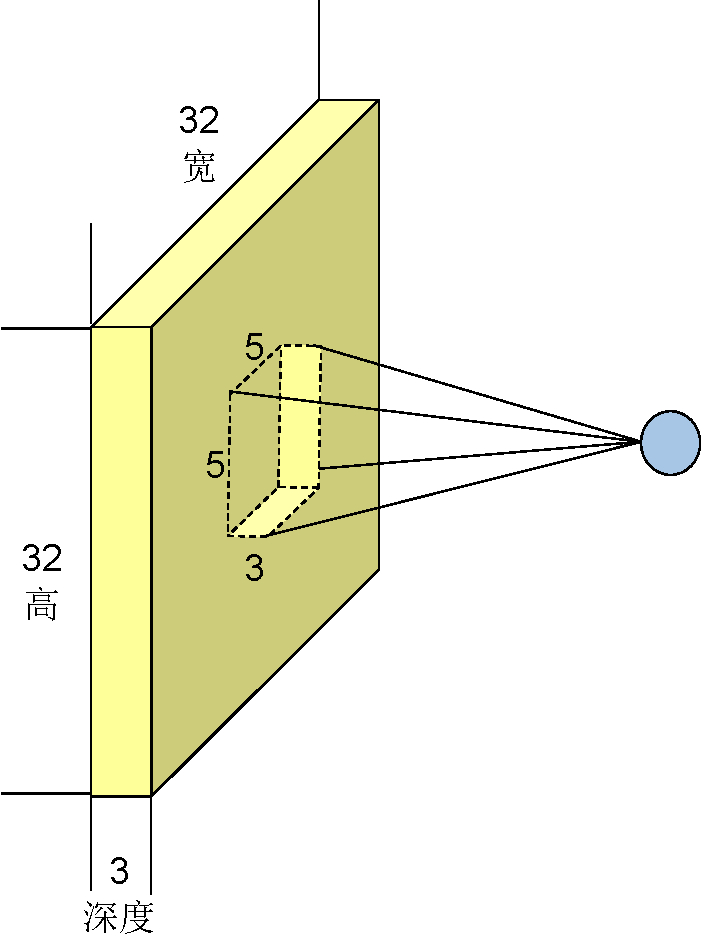
\includegraphics[scale=0.8]{Pictures/CNN/single_layer-crop.pdf}\\
  \caption{局部连接示意图}\label{fig:local_connectivity}
\end{figure*}


以输入层和第一层隐层中的一个神经元节点连接为例, 如图\ref{fig:local_connectivity}所示。 图中黄色区域表示输入, 为32*32*3大小的数据, 比如可表示一张深度为3(3通道), 宽、高均为32的图像。 图中的蓝色圆点表示与输入层相连的一个隐层节点, 连接项由权重参数组成。 和大脑中视觉皮层的接收域(receptive fields)一样, 我们在卷积神经网络的隐层中也设置接收域, 该接收域可以视作一个在输入中进行扫描的线性滤波器, 为了减少参数数量, 该滤波器中的权重参数在输入层中共享。 直观地想, 共享也是有原因的。 因为该接收域的目的是发现输入空间中的一些特定模式, 这是不需要受到检测位置在图像中位置的限制的, 这也解释了为什么CNN网络学出的特征具有平移不变性。 换句话说, 其目的是使我们要找的特定模式与其在输入数据的位置无关。 卷积神经网络中, 我们称该接收域为核(kernel)。 例如图中为5*5的kernel, 深度为3(和通道数相同)。 由于CNN的连接层中共享权值, 所以该节点与输入层相连接的参数个数总共只有5*5*3个。 在输入层中, 从原点(左上角)开始分别向右方和下方扫描, 假如每隔1个像素进行扫描, 每个5*5*3的区域块经5*5*3的kernel卷积得到一个标量, 那么一个数据32*32*3的数据经过卷积也就可以得到一个(32-5+1)*(32-5+1)大小的数据。

对于隐层中有多个节点的情况, 我们在隐层的深度维进行扩展。 假如我们希望隐层有N个节点, 就令隐层的深度为N, 那么隐层大小即为(32-5+1)*(32-5+1)*N。 刚才我们对于输入层每隔一个像素进行一次卷积, 但是为了减小计算复杂度, 我们还可以设置卷积的步长, 也就是每隔多少个元素进行一次卷积操作, 我们称这个步长为stride, 如图\ref{fig:stride}所示为输入大小为7*7的图像, stride为2的情况, 可见此时对应的输出长和宽为(7-3)/2+1。 即给定输入数据大小$(D_h,D_w,D_c)$, kernel大小$(k_h, k_w)$, stride 大小s, 要求卷积神经网络的隐层节点为K, 隐层大小为$((D_h-k_h)/s+1,(D_w-k_w)/s+1,K)$, 有$k_h\times k_w\times D_c\times K$个参数。


\begin{figure*}[htb]
  \centering
  % Requires \usepackage{graphicx}
  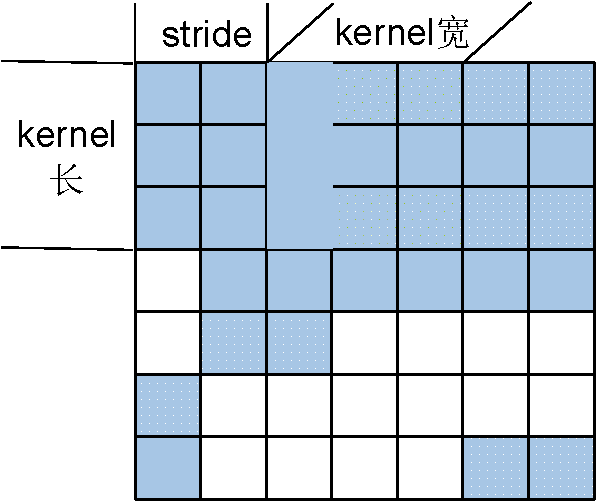
\includegraphics[scale=0.8]{Pictures/CNN/stride-crop.pdf}\\
  \caption{stride示意图}\label{fig:stride}
\end{figure*}




\paragraph{降采样层}





此外, 在卷积神经网络中还有全连接层, 该层间神经元两两连接, 也就是说, 和全连接层相连接的层间权重个数等于两层神经元个数的乘积, 用来增强网络的表达能力。 综上, 一个典型的卷积神经网络如图\ref{fig:lenet}所示。 图为Yan Lecun的为MNIST数据集设计的卷积神经网络。 著名的手写MNIST数据集\cite{lecun1998mnist} 有60000个训练数据和10000个测试数据, 样本大小为32*32, 均为数字0~9, 共10类。

\begin{figure*}[htb]
  \centering
  % Requires \usepackage{graphicx}
  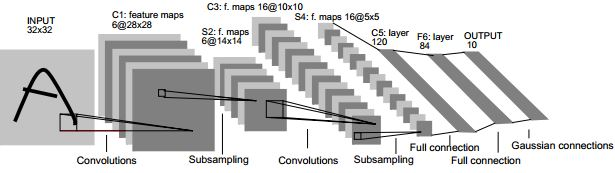
\includegraphics[scale=0.8]{Pictures/CNN/lenet.jpg}\\
  \caption{lenet}\label{fig:lenet}
\end{figure*}






\subsection{CNN的训练}

CNN模型通常用随机梯度下降\cite{nemirovski1978cezari}算法进行优化。 随机梯度下降算法源于随机优化。 随机优化在统计学习理论中非常常见, 即求参数$\theta$来最小化loss的期望。


\begin{equation}
\label{Eq:stocastic_optimization}
	\theta^* = arg min_{\theta} E(L(f(\theta,x),y))
\end{equation}


在线学习中有一个简单算法求这样的$\theta$, 叫做在线梯度下降\cite{zinkevich2003online}: 在每一步迭代中, 按式\ref{Eq:online_gd}更新权重, 其中$\theta_k$为第k步的$\theta$值, $\eta$为学习率。


\begin{equation}
\label{Eq:online_gd}
	\theta_{k+1} = \theta_k - \eta g_k
\end{equation}

也就是更新方向为第k步时梯度下降最快的方向。 这种把数据看做一个源源不断的流数据, 每一轮(epoch)只对其中一部分数据进行更新的方法叫做随机梯度下降(Stochastic Gradient Descent, SGD)。 2006年, Mike O'Neill 在MNIST上训练CNN, 采用4个隐层, 共3215个隐层神经元节点, 134066个权重参数, 184974条网络连接(网络连接数大于权重参数, 因为网络中有两个卷积层, 其中是共享权值的)。 










\section{ConvP300Net}\label{sec:cnn_configure}

\subsection{任务描述}

\subsection{网络结构}

\section{实验结果及实现}\label{sec:cnn_experiment}













